\usepackage{tikz}\begin{subsectionframemod}{Proposed Approaches}
    \begin{overlayarea}{\textwidth}{\textheight}
        \vspace{2mm}
        \bfalert{Main principle:} integrate prototypical networks inside Faster R-CNN.
        \vspace{2mm}
        \begin{overlayarea}{\textwidth}{0.3\textheight}
            \begin{columns}[T]
            
                \begin{column}{0.5\textwidth}
                    \only<2->{
                    \alert{RPN:} multi-class prototypes but only outputs objectness score (i.e. binary classification).
    
                    \centering
                    \begin{minipage}{0.99\textwidth}
                        \centering
                        \begin{equation*}
                            o_{j} = \max\limits_{c \in C_i} \exp\Big(\frac{-d(z_{j}, p_c)^2}{2\sigma^2}\Big)
                        \end{equation*}
                    \end{minipage}
                    }
                \end{column}
                
                \begin{column}{0.5\textwidth}
                    \only<3>{
                    \alert{Classification head:} prototypical networks attribute class scores to RoI extracted from RPN boxes \parencite{karlinsky2019repmet}.
    
                    \centering
                    \begin{minipage}{0.99\textwidth}
                        \begin{equation*}
                            p(c |x_{j,a}) =\frac{\exp\Big(\frac{-d(z_{j}, p_c)^2}{2\sigma^2}\Big)}{\sum\limits_{c' \in C_i \cup \{\varnothing\}} \exp\Big(\frac{-d(z_{j}, p_{c'})^2}{2\sigma^2}\Big)}
                        \end{equation*}
                    \end{minipage}
                    }
                \end{column}
            
            
            
            \end{columns}
        \end{overlayarea}

        \vspace{0mm}
        
        \begin{figure}
            \centering
            \begin{tikzpicture}
                \only<2->{
                    \node[anchor=south west, inner sep=0] (image) at (0,0) {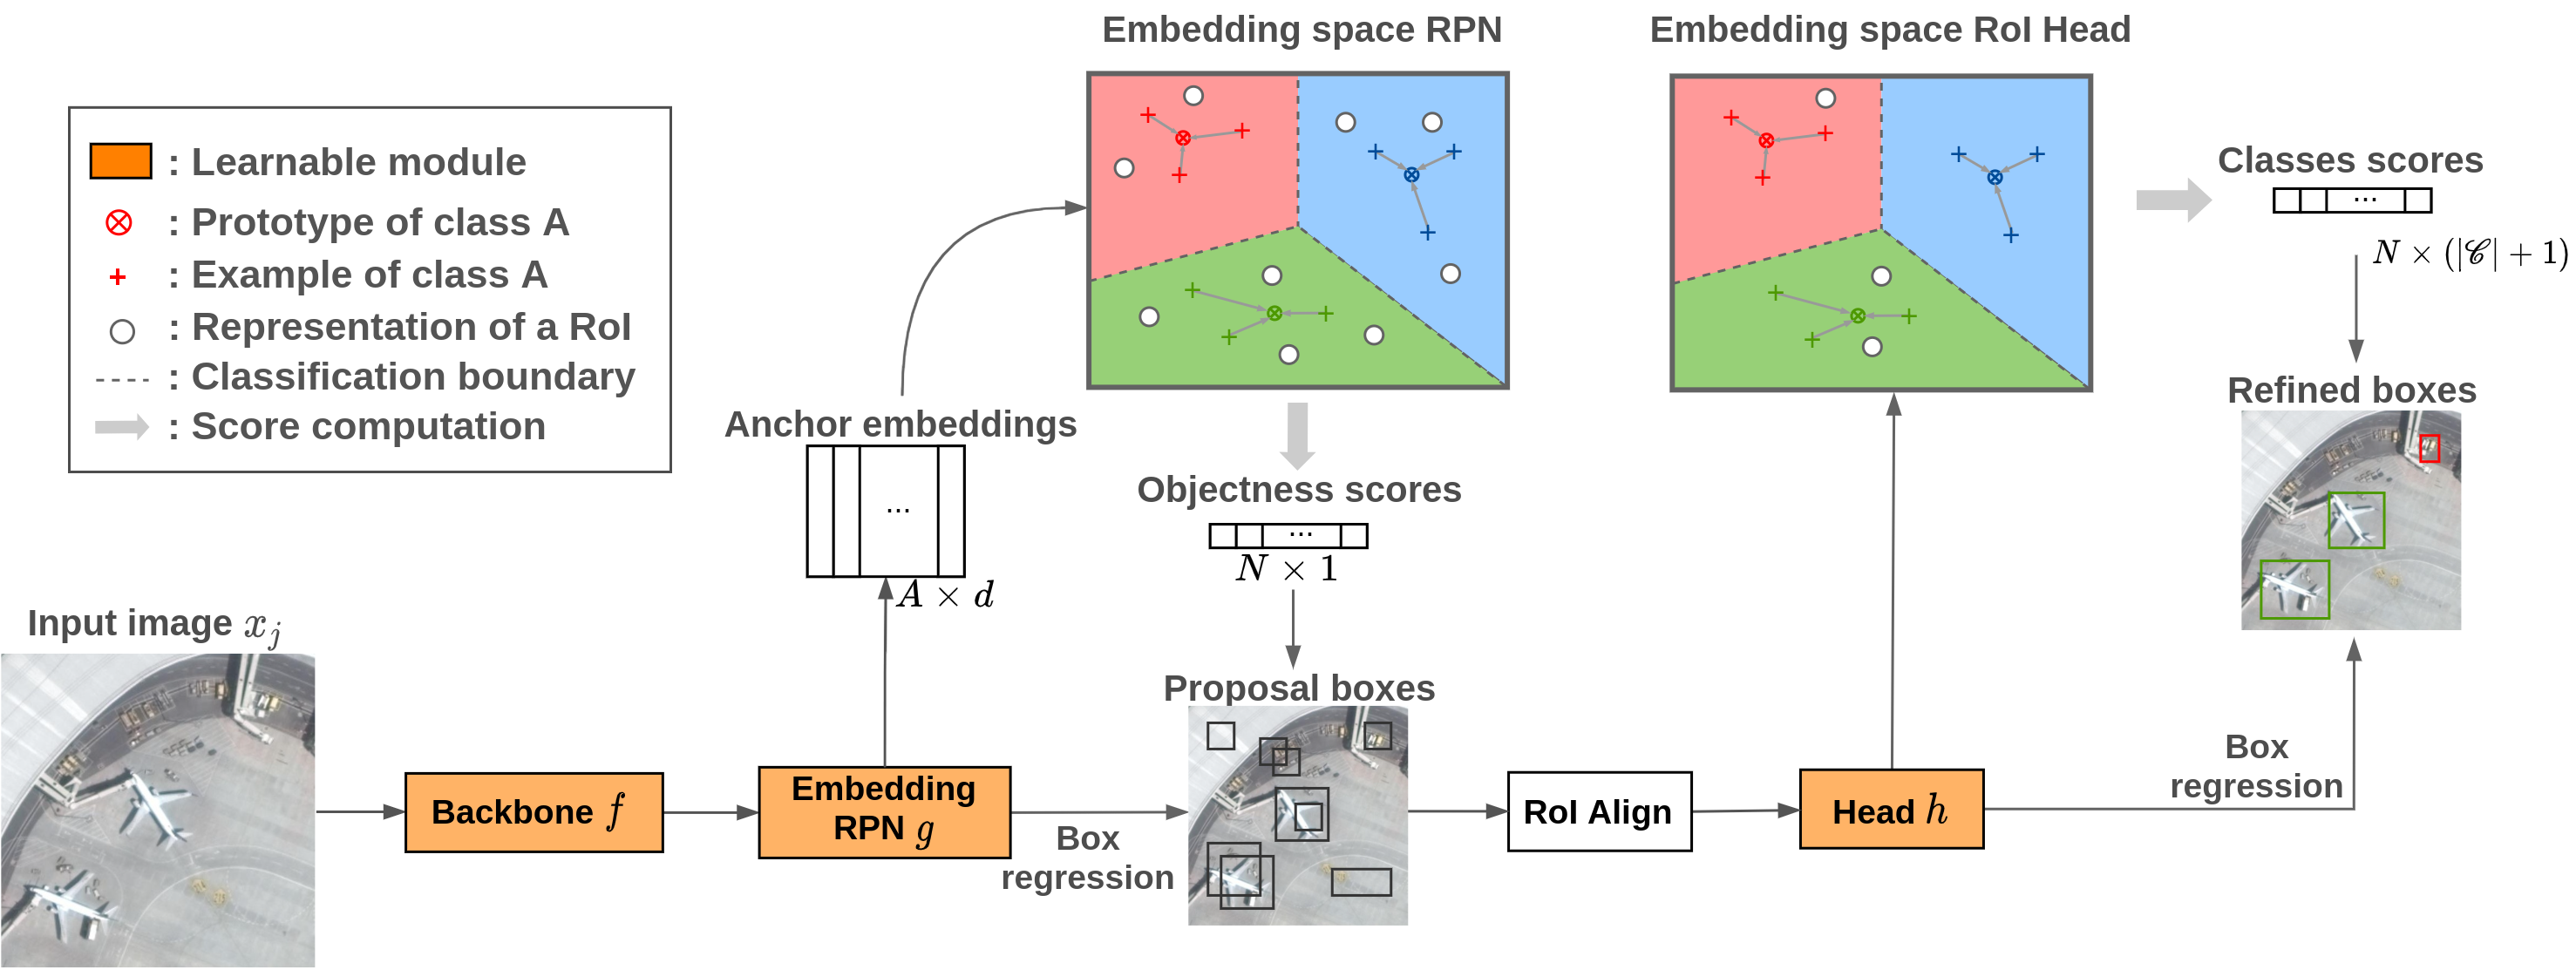
\includegraphics[width=0.95\textwidth]{Figures/prototypical_frcnn_rework.png}};
                }
                \only<2>{
                    \begin{scope}[x={(image.south east)},y={(image.north west)}]
                        \draw[color=black!2, fill=black!2, overlay] (0.62,0.05) rectangle (1,1);
                        \draw[color=black!2, fill=black!2, overlay] (0.55,0.05) rectangle (1,0.25);
                    \end{scope}
                }
                
            \end{tikzpicture}
            \only<2->{
                \vspace{-2mm}
                \caption{Prototypical Faster-RCNN architecture.}
            }
            
        \end{figure}
    
        
    \end{overlayarea}
\end{subsectionframemod}